% This is a LaTeX thesis template for Monash University.
% to be used with Rmarkdown
% This template was produced by Rob Hyndman
% Version: 6 September 2016

\documentclass{monashthesis}

%%%%%%%%%%%%%%%%%%%%%%%%%%%%%%%%%%%%%%%%%%%%%%%%%%%%%%%%%%%%%%%
% Add any LaTeX packages and other preamble here if required
%%%%%%%%%%%%%%%%%%%%%%%%%%%%%%%%%%%%%%%%%%%%%%%%%%%%%%%%%%%%%%%

\author{Stephanie Rose Kobakian}
\title{New algorithms for effectively visualising Australian spatio-temporal disease data.}
\degrees{B.Comm. and B.Eco., Monash University}
\def\degreetitle{Master of Philosophy (Statistics)}
% Add subject and keywords below
\hypersetup{
     %pdfsubject={The Subject},
     %pdfkeywords={Some Keywords},
     pdfauthor={Stephanie Rose Kobakian},
     pdftitle={New algorithms for effectively visualising Australian spatio-temporal disease data.},
     pdfproducer={Bookdown with LaTeX}
}


\bibliography{thesisrefs}

\begin{document}

\pagenumbering{roman}

\titlepage

{\setstretch{1.2}\sf\tighttoc\doublespacing}

\hypertarget{copyright-notice}{%
\chapter*{Copyright notice}\label{copyright-notice}}
\addcontentsline{toc}{chapter}{Copyright notice}

\textcopyright { } \authorname~(\number\the\year).

I certify that I have made all reasonable efforts to secure copyright permissions for third-party content included in this thesis and have not knowingly added copyright content to my work without the owner's permission.

\newpage

\hypertarget{abstract}{%
\chapter*{Abstract}\label{abstract}}
\addcontentsline{toc}{chapter}{Abstract}

The Australian population has congregated in the capital cities and significant cities in each state. This pattern has resulted in very dense population centers and sparsely populated rural areas. The relationship between the Australian population and the geographic area they live on results in a heterogeneous distribution of the map space. The goal of many spatial visualisations is to gain a broad perspective of the values of statistics over the Australian population. However, the use of most mapping techniques can mislead, as the use of geographical areas unequally presents the spatial distribution of a dataset.

The algorithm presented in this thesis will take geospatial areas in the form of polygons and create an alternative graphical display of a spatial distribution. This algorithm takes a set of polygons and creates a map of tessellated hexagons, representing a single geographical area with a single hexagon. It arranges them to replicate spatial relationships of geographic areas in each city. The hexagon tile map visualisation produced by the algorithm is contrasted with the traditional choropleth map.
The package sugarbag \autocite{sugarbag} implements the algorithm for the statistical software R \autocite{R}.

Using animations will allow us to control how people transform a recognisable map of Australia, or the cities within, into a more sound map for inference. Animation is gaining popularity as access to computing power is increasing the amount of applications.

Keywords: maps; statistics; geospatial statistics; visual inference;
\newpage

\hypertarget{declaration}{%
\chapter*{Declaration}\label{declaration}}
\addcontentsline{toc}{chapter}{Declaration}

\emph{(Thesis including published works declaration)}

I hereby declare that this thesis contains no material which has been accepted for the award of any other degree or diploma at any university or equivalent institution and that, to the best of my knowledge and belief, this thesis contains no material previously published or written by another person, except where due reference is made in the text of the thesis.

This thesis includes three original papers submitted to peer reviewed journals. The core theme of the thesis is spatial visualisations. The ideas, development and writing up of all the papers in the thesis were the principal responsibility of myself, the student, working within the Faculty of Science and Engineering under the supervision of DProf. Kerrie Mengersen and Dr.~Earl Duncan. It was also created under the supervision of the external supervisor Prof.~Dianne Cook.

I have not renumbered sections of submitted or published papers in order to generate a consistent presentation within the thesis.

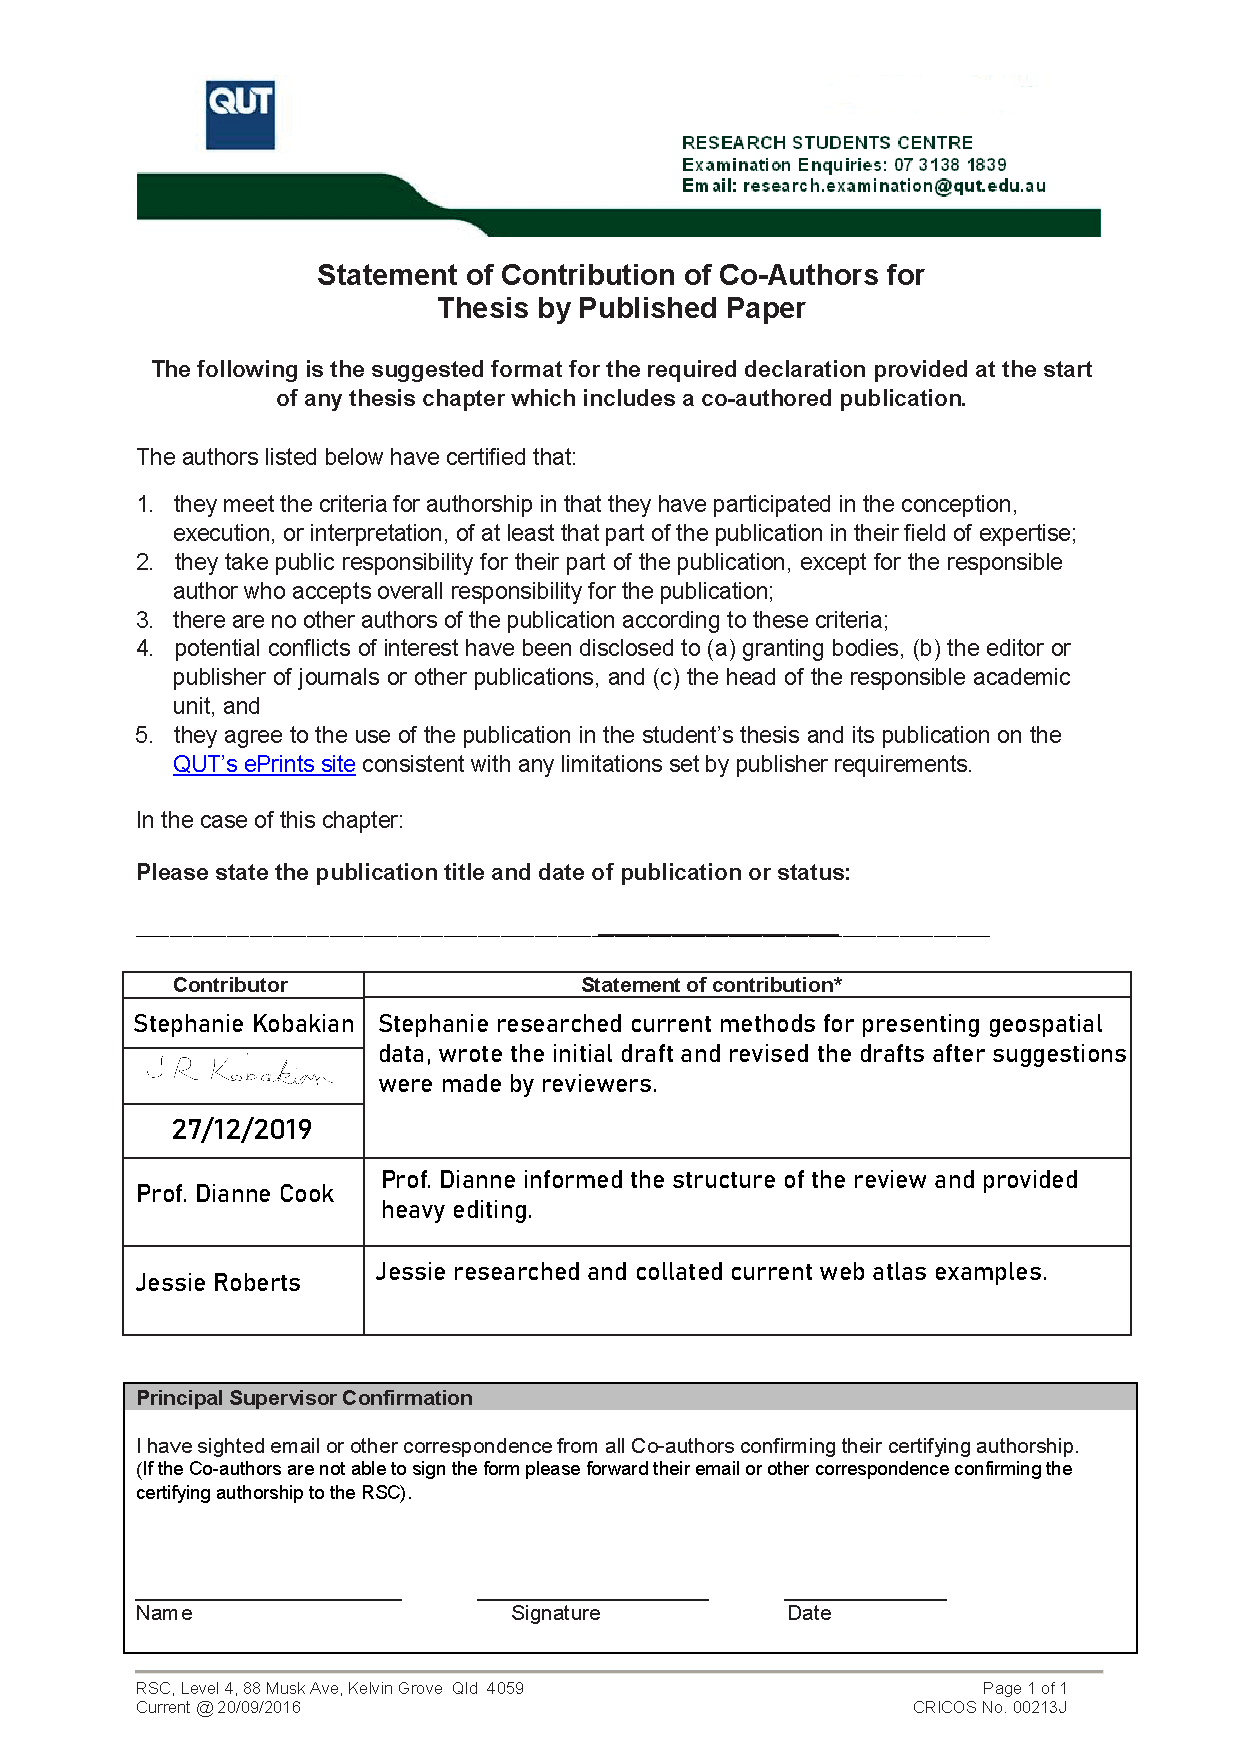
\includepdf[pages = {1-}, scale=1]{statement-of-contribution.pdf}

\hypertarget{acknowledgements}{%
\chapter*{Acknowledgements}\label{acknowledgements}}
\addcontentsline{toc}{chapter}{Acknowledgements}

We would like to acknowledge Dr Earl Duncan (Research Associate at ARC Centre of Excellence for Mathematical \& Statistical Frontiers, QUT). His time and effort given to edit and comment on this paper was invaluable.

We thank Dr Susanna Cramb (Spatial Modeller, Cancer Council Queensland) and Dr Peter Baade (Senior Research Fellow, Cancer Council Queensland) for providing the opportunity to cover this exploration of disease mapping methods in writing.
This literature review would not be possible without the opportunity provided by Queensland University of Technology, and Cancer Council Queensland, and the roles of Professor Kerrie Mengersen (Professor of Statistics, Science and Engineering Faculty, QUT) and Dr Earl Duncan in contributing to the Australian Cancer Atlas and supervision of Stephanie's Research Masters.

It was in the development of this online cancer atlas that methods for disease map displays, and visual communication strategies were explored. We are thankful for the opportunity to write about these visualizations and the situations in which they are appropriate.

Several R \autocite{R} packages were used to produce this paper.
For data analysis the tidyverse package \autocite{tidyverse} provided many useful functions.
ggplot2 package \autocite{ggplot2} was used to create maps, with RColorBrewer package \autocite{RColorBrewer} providing additional color palettes and ggthemes \autocite{ggthemes} package providing themes.
The png package \autocite{png} was used to access png images taken from online web atlases, cowplot package \autocite{cowplot} was used to arrange these plots into grouped images.

The following packages were used to create transformations from the sf \autocite{sf} geographical shapes of the states of America \autocite{spData} and the Australian Statistical Areas (Level 3):
The cartogram \autocite{cartogram} package creates contiguous, non-contiguous and Dorling cartograms.
Hexagon tile map displays were created using the sugarbag package \autocite{sugarbag}.

\hypertarget{preface}{%
\chapter*{Preface}\label{preface}}
\addcontentsline{toc}{chapter}{Preface}

\begin{enumerate}
\def\labelenumi{\arabic{enumi}.}
\tightlist
\item
  The literature review exploring current practice for visualisaing spatial data in Chapter two has been submitted to the journal \emph{Annals of Cancer Epidemiology} for possible publication.
\end{enumerate}

\begin{enumerate}
\def\labelenumi{\arabic{enumi}.}
\setcounter{enumi}{1}
\item
  The details of the algoirthm documented in Chapter three have been submitted to the \emph{Journal of Statistical Software}.
\item
  The details of the visual inference testing is documented in Chapter four has been submitted to the \emph{IEEE Transactions of Visualisation and Computer Graphics} under the title ``Which is Better: a Choropleth Map or Hexagon Tile Map? A comparison using visual inference.''
\end{enumerate}

\begin{enumerate}
\def\labelenumi{\arabic{enumi}.}
\setcounter{enumi}{3}
\tightlist
\item
  The code for the algorithm documented in Chapter three has been submitted to \emph{CRAN} as the package sugarbag.
\end{enumerate}

Stephanie Kobakian and Dianne Cook (2019). sugarbag: Create Tessellated
Hexagon Maps. \url{https://srkobakian.github.io/sugarbag/},
\url{https://github.com/srkobakian/sugarbag}.

\clearpage\pagenumbering{arabic}\setcounter{page}{0}

\hypertarget{ch:intro}{%
\chapter{Introduction}\label{ch:intro}}

There are many visualisation methods used to present geospatial data. The design of the visualisation chosen can hinder or improve the communication of the spatial distribution. A choropleth map is the most common display used to present geographical data.Maps contribute to understanding spatial distributions of disease occurrence, and locating disease clusters. Disease data is often aggregated by political areas. One reason for this is privacy, another the responsibility on the political entity to respond. The typical visualisation for aggregated spatial data is a choropleth map, where areas are coloured by the numerical value.

Choropleth maps do a disservice to the map reader, as the attention of the map user is distributed according to the size of the area. Using a choropleth map to get a broad perspective of Australia can be misleading, when the use of geographical areas misrepresents the spatial distribution of a dataset. This is not practical if each area is considered equally important. In Australia, the population is not equally dispersed across the geographic map base.
Instead, the communities are densely populated in the inner city areas, especially around the capital cities. There are several visualisation methods that have been developed to emphasise the population dense areas. These alternatives should be considered when planning the communication of geospatial statistics. Visualisations should be chosen to best represent the spatial distribution, The work is motivated by the Cancer Atlas of Australia,
which presents the spatial patterns of many cancers in Australia. The aim of this thesis is to contribute an algorithm that creates effective visualisations for the communication of geospatial population statistics.

\hypertarget{the-australian-cancer-atlas}{%
\section{The Australian Cancer Atlas}\label{the-australian-cancer-atlas}}

This work was motivated by the Australian Cancer Atlas. An online, interactive web tool for exploring the impact of cancer on Australian communities. The prominent display used by the Australian Cancer Atlas is a visualisation of Incidence Rates or Excess Death Rates. The set of geographic units used is Australian Statisical Areas, at Level 2. There are almost 2,200 individual areas, ranging in size from

The choropleth map display used in the Australian Cancer Atlas is familiar to the general public of Australia. It is appropriate to use this display as users can orient themselves on the map base and find geographic areas relevant to them.
However, when the intention of the map user is to convey the whole spatial distribution the information derived visually from the colours can be misleading.
The rural areas are over emphasised, and the densely populated inner city areas are not given enough attention.

\hypertarget{visual-inference}{%
\section{Visual Inference}\label{visual-inference}}

Visual inference will be used to determine if the communication of population geospatial statistics is more effective when using an alternative display.
Buja et al \autocite{GIIV} provide the `lineup' protocol as a formal framework for testing visual statistical methods. Implementing this framework will allow new alternative visualisation method to be tested.

The lineup protocol will be used to test if a visualisation is effective, a visualisation displaying a real population based distribution can be hidden in a collection of visualisations that display null distributions \autocite{chowd}.
It takes inspiration from a police lineup.
The witness in this regard is a participant recruited from a crowdsource platform, such as Figure-Eight.
The visualisation containing a real distribution is considered the `accused'.
It is put in a lineup of innocent displays that do not show a real population based distribution.
If the `witness' chooses the `accussed' as different from the innocent plots, it can be considered that there is a specific pattern displayed that is not present in the others.
In this protocol, the null hypothesis can be rejected in favour of the alternative when it is chosen in the lineup. The null hypothesis fails to be rejected when it is not selected in the linup.

\hypertarget{aims-and-objectives}{%
\section{Aims and Objectives}\label{aims-and-objectives}}

This work aims to provide a solution to presenting geospatial data regarding populations.
It considers the visualisation methods developed over the past two centuries that shift the focus from the geographic map base.

\begin{enumerate}
\def\labelenumi{\arabic{enumi}.}
\item
  \emph{Algorithm for creating hexagon tile maps of Australia:} The algorithm will take geospatial areas and create an alternative visualisation of the spatially distribution.
\item
  \emph{Test the effectiveness of the hexagon tile map relative to the choropleth map:} The hexagon tile map produced by the algorithm will be contrasted with the traditional choropleth map, applying the same colour methods to represent the data. The maps will be used in an experiment to test the effectiveness by asking for users to spot spatial distributions.
\item
  \emph{Communicating the relationship between the hexmap and choropleth map through animation:} Maximise the benefits of both displays when communicating to the public. The use of animations may control how people follow a recognisable map of Australia into an alternative visualisation for inference.
\end{enumerate}

\hypertarget{research-contributions}{%
\section{Research Contributions}\label{research-contributions}}

This research contributes a new algorithm for creating hexagon tile map displays. It contributes an R \autocite{R} package which implements the algorithm and allows R users to create their own visualisations.
It presents a case study that contributes to a growing field of visual inference studies, applied to spatial data by comparing a choropleth map to a hexagon tile map display.
It also shows how it can be used in practice to effectively communicate cancer distributions.

\hypertarget{thesis-structure}{%
\section{Thesis Structure}\label{thesis-structure}}

The thesis is structured as follows: Chapter two contains a literature review.
The literature reviews considers the current peer reviewed literature and published books that explore spatial distributions of cancer across the globe.
It also considers how to evaluate the visualisation methods used for spatial data.

Chapter three explores the algorithm to create hexagon tile maps and the code used to create a small example of Tasmania in Australia.
Chapter four is a visual inference study that contains the methods and results that compare the use of a choropleth map and a hexagon tile map on the same data sets.
Chapter five provides a conclusion of the results of the visual inference study and how the hexagon tile map may be used in practice.

\hypertarget{ch:literature}{%
\chapter{Literature Review}\label{ch:literature}}

\includepdf[pages = {1-33}, scale=1]{literature.pdf}

\hypertarget{ch:algorithm}{%
\chapter{Algorithm}\label{ch:algorithm}}

\includepdf[pages = {1-11}, scale=1]{algorithm.pdf}

\hypertarget{ch:experiment}{%
\chapter{Visual Inference Study}\label{ch:experiment}}

\includepdf[pages = {1-}, scale=1]{experiment.pdf}

\hypertarget{discussion}{%
\chapter{Discussion}\label{discussion}}

Visualisation methods have improved in iterations over many years. Cartograms showed great promise and several algorithms were presented to create cartograms in the 1960s and 1970s.
The introduction of computer assisted cartogram techniques were developed in the 1970s and 1980s. Dorling \autocite{TVSSS}, \autocite{ACTUC} introduced several alternative visualisation methods and their use has had a profound impact in the communication of data with population related distributions.
Nusrat and Kobourov provide examples for techniques to evaulate the statistical, geographical, and topological accuracy of alternative visualisation displays.

\hypertarget{conclusion}{%
\chapter{Conclusion}\label{conclusion}}

The goal of this thesis was to present an alternative visualisation method for spatial data. This thesis has provided a new algorithm to present spatial distributions of disease data, and includes an R code \autocite{R} implementation. The spatial data sets that will be effectively communicated by this display will likely have population related distributions. The hexagon tile map display will represent each area equally on the map space to effectively convey the spatial distribution of the set.

The hexagon tile map alternative visualisation method solves the misprepresentation problem of choropleth displays of geographic data sets that contain a substantial amounts of areas. This algorithm is accessible to all R users, in a set of simple functions. It can be applied to any set of areas in an \texttt{sf} \autocite{sf} object. The several working example helps users to apply the functions to their own data sets.

The method outputs data sets to users that can easily be used to create animations between a choropleth and hexagon tile map display. Linking the familiar geography to the effective display for understanding the distribution across many heterogeneous geographic regions.

The effectiveness of the hexagon tile map has been proved by the visual inference study. It showed that participants could recognise the data display in the set of null distributions more frequently when viewing a hexagon tile map display. The choropleth map display is still effective for distributions that are directly related to the geography, such as the North-West to South-East distribution used in the study.
This has expanded the applications of visual inference studies in a spatial data context.

Future work will include expanding on criteria to evaulate the hexagon tile maps produced by the algorithm. The methods to evaluate the alternative displays have not been thoroughly explored in this thesis.
This framework will be used to create relevant tests that contrast the use of the map area, and changes in the visual statistics when the parameter of the hexagon tile map algorithm are altered.

This work has contributed a new visualisation for spatial data sets. The spatial distributions of cancer burden for different types of cancers largely relates to the population rather than the geography. The alternative visualisation method highlights the communities, and the hexagon tile map may be implemented in future iterations of the Australian Cancer Atlas to improve the communication of spatial patterns of cancer burden on Australian communities. For wide use by map creators and those interested in alternative visual diaplays, the code implementation has been provided to any R user with examples and documentation.
This work has also contributed to the literature of visual inference studies, by using the ``lineup'' protocol developed by Buja et al.~and used by Wickham, Cook and Hofmann \autocite{GIIV}, \autocite{GTPCCD}. This example showed there was a difference in the rate of pattern recognition when participants saw competing spatial map displays.

To communicate human related spatial patterns of disease, map creators should consider the use of alternative displays. The hexagon tile map display has proven effective in this thesis for communicating spatial distributions in sets of heterogeneous geographic units. This thesis provides a practical guide for map creators communicating spatial displays of cancer data in Australia.

\appendix

\includepdf[pages = {1-}, scale=1]{Study_1.pdf}

\hypertarget{ch:ethics}{%
\chapter{Ethics Approval}\label{ch:ethics}}

\includepdf[pages = {1-}, scale=1]{Ethics_1.pdf}

\printbibliography[heading=bibintoc]



\end{document}
